%
% monopol.tex -- Monopol Niveaulinien
%
% (c) 2017 Prof Dr Andreas Müller, Hochschule Rapperswil
%
\documentclass[tikz]{standalone}
\usepackage{times}
\usepackage{txfonts}
\usepackage{fp}
\usepackage{ifthen}
\usepackage[utf8]{inputenc}
\usetikzlibrary{arrows,intersections}
\usetikzlibrary{fixedpointarithmetic}
\begin{document}
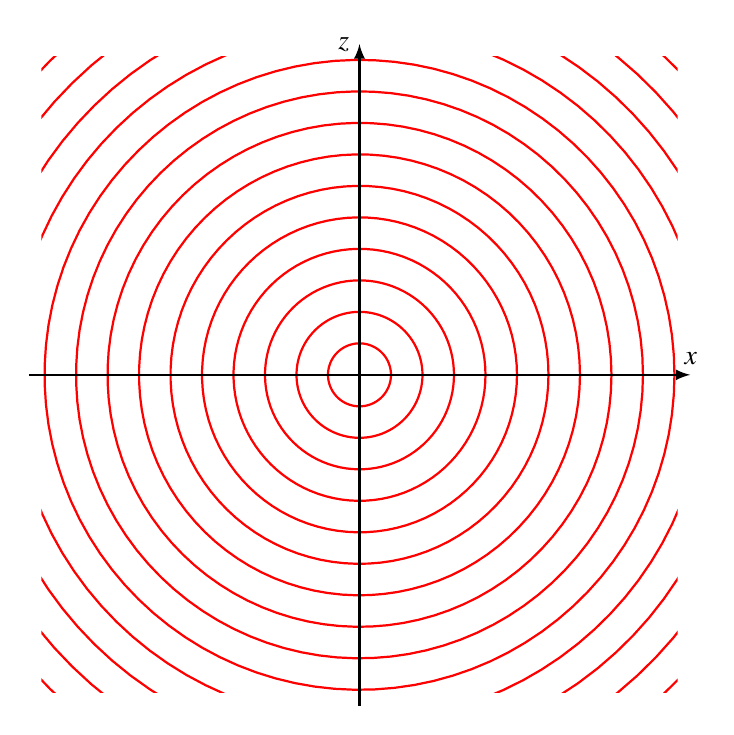
\begin{tikzpicture}[>=latex, thick, scale=2]

\begin{scope}
\clip (-2.02,-2.02) rectangle (2.02,2.02);
\foreach \c in {1,...,30}
{
	\draw[domain=0:360,samples=100,red] plot ({\x}:{\c/5});
}
\end{scope}

\draw[->] (-2.1,0)--(2.1,0) coordinate[label={above:$x$}];
\draw[->] (0,-2.1)--(0,2.1) coordinate[label={left:$z$}];

\end{tikzpicture}
\end{document}
